%%
%\listfiles
%\documentclass[%
% reprint,%
%secnumarabic,%
% amssymb, amsmath,%
% aip,cha,%
%groupedaddress,%
%frontmatterverbose,
%]{revtex4-1}
\documentclass[twocolumn,amsmath,amssymb,showpacs,pre,nofootinbib,superscriptaddress]{revtex4-1} %,preprint,jcp
% \documentclass[journal=jacsat,manuscript=article]{achemso}

\bibstyle{apsrev}
%\usepackage{docs}%
\usepackage{bm}%
\usepackage{graphicx}
%\usepackage{subcaption}
\usepackage{tikz}
\usepackage{ulem}
\usepackage{color}
\usepackage{xcolor}
\usepackage{physics}
\usepackage[colorlinks=true,linkcolor=blue]{hyperref}%
%\nofiles
\expandafter\ifx\csname package@font\endcsname\relax\else
 \expandafter\expandafter
 \expandafter\usepackage
 \expandafter\expandafter
 \expandafter{\csname package@font\endcsname}%
\fi
\hyphenation{title}
\newcommand{\figloc}[1]{Figures/#1}

\begin{document}

\definecolor{pyblue}{HTML}{1F77B4}
\definecolor{pyorange}{HTML}{FF7F0C}
\definecolor{pygreen}{HTML}{2CA02C}
\definecolor{pyred}{HTML}{D62728}

\title{Droplet coalescence assisted with surface tension gardients}

\author{S. Zitz}
\email{zitz@ruc.dk}
 \affiliation{IMFUFA, Department of Science and Environment,\\ Roskilde University, Postbox 260, DK-4000 Roskilde, Denmark}%
 \affiliation{Department of Chemical and Biological Engineering, Friedrich-Alexander-Universit\"at Erlangen-N\"urnberg, F\"{u}rther Stra{\ss}e 248, 90429 N\"{u}rnberg, Germany}%
 \author{T. Richter}%
%\email{t.richter@fz-juelich.de}
 \affiliation{Helmholtz Institute Erlangen-N\"urnberg for Renewable Energy,\\
  Forschungszentrum J\"ulich,
  F\"urther Strasse 248, 90429 N\"urnberg, Germany}%
  \affiliation{Department of Physics, Friedrich-Alexander-Universität Erlangen-Nürnberg, \\Fürther Straße 248, 90429 Nürnberg, Germany}%
 \author{K. Missios}%
%\email{missios@ruc.dk}
 \affiliation{IMFUFA, Department of Science and Environment,\\ Roskilde University, Postbox 260, DK-4000 Roskilde, Denmark}%
%\author{H. Scheufler}%
%\email{henning.scheufler@dlr.de}
%\affiliation{DLR German Aerospace Center,\\ Institute of Space Systems, 28359 Bremen, Germany}%
 \author{J. P. Roenby}%
\email{johan@ruc.dk}
 \affiliation{IMFUFA, Department of Science and Environment,\\ Roskilde University, Postbox 260, DK-4000 Roskilde, Denmark}%
\date{\today}

\begin{abstract}
We numerically study the coalescence dynamics of two sessile droplets.
The droplets are placed on top of a rigid substrate with a contact angle of $\theta_{eq.} = \pi/9$. 
Having a highly wettable substrate ($\theta_{eq} \ll \pi/2$) theory predicts that the bridge height ($h_0$) scales according to $h_0(t) \propto t^{2/3}.$
This behavior can be altered with e.g. surface tension gradients ($\partial\gamma \neq 0$). 
These gradients appear for example using heating devices, surfactants or having different but miscible liquids.
Instead of coalescence, these gradients can lead to a stable two droplet state. 
In this work, we focus on two aspects of this problem.
First being the concrete choice of the surface tension gradient.
And second, the reduction of scale towards a regime in which the disjoining pressure is important. 
To do so, we introduce a disjoining pressure and couple it to the local surface tension.
Showing that coalescence can be suppressed but also the theoretical $2/3$ powerlaw emerges for a vanishing gradient.
Between those two extrema we find intermediate bridge growth and asymmetric coalescence.
\end{abstract}

\maketitle

\newcommand{\ts}{\textsuperscript}

\section{Introduction}\label{sec:intro}
The coalescence or non-coalescens of liquid droplets is an interesting problem to study. 
Both scenarios can be observed in many instances of our every day life and in various industrial processes.
Coalescence of sessile droplets happens, for example, when vapor condenses on the lid of a pot.
Starting with the nucleation of small droplets, which quickly assemble in larger drops either naturally~\cite{PhysRevA.43.1906} or due to artificial factors such as surface structure or patterning~\cite{C1SM06219K}. 
This effect can effectively be used in so-called fog harvesting devices. 
These devices can be an effective source for liquid water as they collect ambient water vapor~\cite{zhang2015inkjet, shi2018fog}.
Apart from fog harvesting, coalescence or rather the control of it plays an important part in inkjet printing and printable electronics~\cite{jo2009evaluation, singh2010inkjet, Kim_2005, Luechinger_2008}.
But also in various microfluidic devices for mixing purposes at low Reynolds numbers ($Re < 1$). 
The coalescence of droplets in this regime can serve as an effective mixing technique~\cite{https://doi.org/10.1002/pen.760352206, doi:10.1063/1.858199}. 

On the other hand, there are many applications that require droplets not to coalesce.
In hot summer days, a fine water spray can help the body to cool down.
Single, small droplets advect the heat from the body and transfer it into the surrounding fluid (air)~\cite{kim2007spray}.
% Cooling hot, structures, as such structures near boiling point is another issue which ~\cite{JIA2003829}.
Apart from cooling, emulsions are an illustrative example of systems where droplets should not coalesce.
Thinking about Mayonnaise where due to vigorously stirring the oil breaks up in small droplets that mix with the water of the egg yolk.
Proteins and additions like mustard stabilize this state and keep the oil from coalescing, which has a significant effect on the rheology of this mixture~\cite{harrison1985factors, DEPREE2001157}.

Independent of these examples, droplet coalescence has attracted much attention in the past two decades, see refs.~\cite{eggers_lister_stone_1999, duchemin_eggers_josserand_2003, PhysRevLett.95.164503, PhysRevLett.106.114501, doi:10.1063/1.4828721}. 
The basic theoretical arguments, therefore the minimization of surface are and minimization of curvature due to capillarity, hold true for even more complex scenarios. 
Within the same assumptions, one can explain the coalescence of liquid lenses~\cite{PhysRevLett.124.194502} or quasi 2D liquids~\cite{klopp2020self, doi:10.1021/acs.langmuir.0c02139}.
What is common to all studies is the fact that the equilibrium state is one where the two droplets have coalesced.
This is of course in agreement with a minimized surface area and minimal curvature.
Interestingly, this doesn't always apply.

Quite recently, Kern et al. have shown that viscoplasticity can lead to stable twin drop states~\cite{https://doi.org/10.48550/arxiv.2203.15617}.
What has been known for some time however is that a surface tension gradient influences the coalescence. 
This has been shown by Karpitschka et al. in experiments with different miscible liquids~\cite{PhysRevLett.109.066103, doi:10.1021/la500459v, karpitschka2014sharp, bruning2018delayed}, but has been studies with numerical experiments as well by Bocia and Bestehorn~\cite{PhysRevE.82.036312, borcia2011coalescence}.
In their work, Karpitschka et al. identify an effective Marangoni flow that stabilizes the two droplet system.
We revisit that problem with numerical simulations.
First, we move to the regime where the droplet become small and disjoining pressure can no longer be neglected.
Second, we address the impact of the surface tension beyond the reduction to its absolute contrast.
Therefore, asking if the concrete function of $\gamma(x)$ can turn non-coalescing states into coalescing ones.
Within this framework, we discuss the growth law of the liquid bridge and symmetry of the coalescence.

This paper is organized as follows:
Starting in the next section, Sec.~\ref{sec:theory}, we discuss the underlying theoretical model.
Introducing the thin film equation with an additional term due to the Marangoni flow. 
Followed by our choice for modelling $\Pi(h)$ the disjoining pressure functional, which consists of thickness dependent powerlaw and a wettability component. 
In Sec.~\ref{sec:method} we discuss the numerical method we use to solve the thin film equation from the previous section.
We show how to construct an addition term to account for the flow induced by the Marangoni effect.
Supplying as well the three functions we use for $\gamma(x)$. 
The results are presented and discussed in Sec.~\ref{sec:results}.
Showing, first, coalescence and non-coalescence based on our choice of $\gamma(x)$.
But also showing that a smoothly varying surface tension relaxes the non-coalescence behaviour.
Finally, conclusions and summary are provided in Sec.~\ref{sec:sum_conclu}. 

\section{Theory}\label{sec:theory}
The theoretical approach we use to study this system is the lubrication approximation~\cite{Reynolds, RevModPhys.69.931, PhysRevE.63.011208}.
Applying this approximation to the Navier Stokes yields the thin film equation, which for a singular horizontal dimension reads~\cite{RevModPhys.81.739, RevModPhys.81.1131, THIELE2014399}
\begin{equation}\label{eq:thin_film_simple}
    \partial_t h = \partial_x \left(\frac{h^3}{3\mu}\partial_x p\right),
\end{equation}
where $\frac{h^3}{3\mu}$ is the mobility $m(h)$\footnote{$m(h) = h^3/3\mu$ is true only for a no-slip velocity boundary condition.}, $h(x,t)$ is the thickness of the film at time $t$ and position $x$, $\mu$ is the liquid's viscosity, and $p$ it's pressure.
The pressure accounts for both the surface tension, thus the interface minimization, and the for correct fluid substrate behavior (wetting)~\cite{PhysRevE.100.033313}.
We can therefore write the pressure as
\begin{equation}\label{eq:pressure}
    p = \gamma \partial_x^2 h + \Pi(h),
\end{equation}
where the first term is the Laplacian of the liquid-vapor interface and $\Pi(h)$ is the disjoining pressure~\cite{RevModPhys.69.931, RevModPhys.81.739, Peschka9275, PhysRevE.63.011208},
\begin{equation}\label{eq:disjoin}
    \Pi(h) = K(\gamma,\theta)\left[\left(\frac{h_{\ast}}{h}\right)^n - \left(\frac{h_{\ast}}{h}\right)^m\right].
\end{equation}
The prefactor $K(\gamma,\theta)\propto \gamma(1-\cos(\theta))$ encodes the wettability and as such the equilibrium contact angle $\theta_{\text{eq.}}$.
This prefactor also serves a link from the disjoining pressure to the Hamaker constant ($\mathcal{A}$) with~~\cite{PhysRevE.93.013120, bestehorn20033d, van1988interfacial}
\begin{equation}
    \mathcal{A} = 6\pi h_{\ast}^3 K(\theta).    
\end{equation}
Additionally, $h_{\ast}$ defines the thickness of the precursor layer, therefore the thickness where $\Pi(h_{\ast}) = 0$.
For the reminder of this manuscript, we define $h(x,t) \le h_{\ast}$ as a ``dry'' spot.
The pair of powers $(n,m)$ need to satisfy $n > m$ and $m > 1$ and are chosen to be $(9,3)$, which resembles a  widely adopted model that was first introduced by Schwartz and Eley~\cite{SCHWARTZ1998173, RevModPhys.81.739}.

\begin{figure}
    \centering
    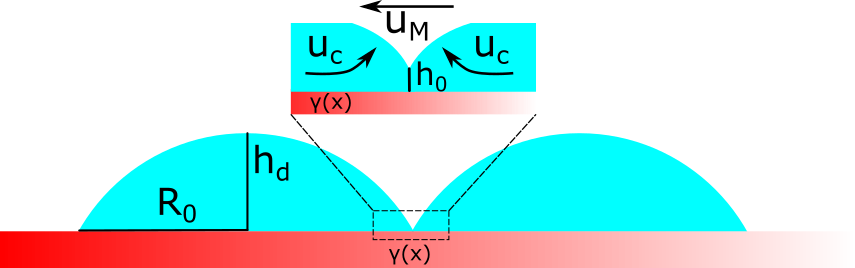
\includegraphics[width=0.48\textwidth]{Figures/setup.png}
    \caption{Schematic setup of the numerical experiment. 
    Two droplets with base radius $R_0$ and maximum height $h_d$ are placed next to each other. 
    They are connected by a liquid bridge with height $h_0$ and subject to a surface tension gradient $\gamma(x)$ .
    The flow has two sizeable contributions, $u_c$ flow due to capillarity and $u_M$ flow due to the Marangoni effect.
    }
    \label{fig:schematics}
\end{figure}
In the presence of a surface tension gradient, Eq.~(\ref{eq:thin_film_simple}) requires an additional term.
This term accounts for an effective Marangoni flow~\cite{doi:10.1021/la500459v, karpitschka2014sharp, bestehorn20033d, doi:10.1021/la960488a}
\begin{equation}\label{eq:thin_with_marangoni}
    \partial_t h = \partial_x \left(\frac{h^3}{3\mu}\partial_x p + \frac{h^2}{2\mu}\partial_x\gamma\right).
\end{equation}
Naturally in case of $\partial_x\gamma = 0$ we retrieve Eq.~(\ref{eq:thin_film_simple}).
These gradients appear due to non-homogenized surfactant concentrations or space resolved heating profiles, e.g. with lasers~\cite{doi:10.1021/la960488a, NIKOLOV2002325, bruning2018delayed, wedershoven2014infrared} or due to different but miscible liquids~\cite{doi:10.1021/la800630w, karpitschka2014sharp, doi:10.1021/la500459v}. 

\subsection{Flows}\label{subsec:flows_theory}
Eq.~(\ref{eq:thin_with_marangoni}) defines the dynamic of the system we are interested in.
Simplifying the equation and setting $\partial\gamma = 0$, we are left with a pure coalescence case.
Following the argumentation of Riegler, Lazar and Eddie et al.~\cite{doi:10.1021/la800630w, PhysRevLett.111.144502} the dynamics is dictated by an strong capillary pressure,
\begin{equation}\label{eq:cap_pressure}
    P_{\text{cap.}} \sim\gamma\kappa \sim \frac{\gamma}{h_0},
\end{equation}
where $\kappa$ is curvature of the liquid vapor interface. 
Having a large curvature at the touching point of the two droplets.
The resulting flow towards the bridge induces a dynamical or ``Bernulli'' pressure
\begin{equation}\label{eq:P_Bernulli}
    P_{\text{iner.}} \sim \rho v^2 \sim \rho\left(\frac{h_0}{t}\right)^2.
\end{equation}
Balancing Eqs.~(\ref{eq:cap_pressure}-\ref{eq:P_Bernulli}) and solving for $h_0$ therefore yields a growth law 
\begin{equation}\label{eq:coal_powerlaw}
    h_0(t) \propto t^{2/3},
\end{equation}
for a constant surface tension with contact angles below $\theta < \pi/2$~\cite{PhysRevLett.111.144502, keller2002breaking}.
Recently, a similar growth law for the coalescence of liquid lenses has been experimentally observed and theoretically validate, see Hack et al.~\cite{PhysRevLett.124.194502}.

The addition of $\partial\gamma \neq 0$ alters the pressure balance.
Riegler and Lazar coupled Eq.~(\ref{eq:P_Bernulli}) to the difference in surface tension~\cite{doi:10.1021/la800630w}
\begin{equation}\label{eq:P_bernulli_riegler}
    P_{B} \sim \rho v^2 \sim \frac{\rho \Delta\gamma^2}{\mu^2}, 
\end{equation}
with the velocity,
\begin{equation}\label{eq:vel_riegler}
    v = \frac{h_0}{\mu}\partial_x\gamma\approx\frac{\Delta\gamma}{4\mu}\theta,
\end{equation}
where $\Delta\gamma = \gamma_1 - \gamma_2$ and $\gamma_i$ are the surface tensions of the two miscible liquids.
Karptischka and Riegler later formulated an elegant theoretical explanation for the flow of the non-coalescing twin droplet state~\cite{PhysRevLett.109.066103}.
Assuming a quasistatic thickness ($\partial_t h \approx 0$) and introducing a constant motion which preserves the droplets.
We proceed similarly, with two differences. 
Considering the disjoining pressure in our derivation, but disregard the velocity term $\propto Ca$.
Starting point is Eq.~(\ref{eq:thin_with_marangoni}) in the limit $\partial_t h \approx 0$, 
\begin{equation}\label{eq:pressure_noncoal}
    \frac{h^3}{3\mu}\partial_x p + \frac{h^2}{2\mu}\partial_x\gamma = 0.
\end{equation}
Solving the above equation for the pressure and inserting Eq.~(\ref{eq:pressure}) we have
\begin{equation}\label{eq:thin_film_quasistatic_pressure}
    \partial_x (\gamma\partial_x^2 h + \Pi(h)) = - \frac{3}{2 h}\partial_x\gamma,
\end{equation}
with $\partial_x\Pi(h)$ on the left-hand side.
Splitting the disjoining pressure into a component depending only on surface tension (\textit{and contact angle}) $K(\gamma)$ and one depending on thickness only $H(h)$ we can readily perform the derivative
\begin{align}\label{eq:disj_derivative1}
    \partial_x\Pi(h) &= \partial_x (K(\gamma)H(h)) \nonumber\\
    &= H(h)\partial_\gamma K(\gamma)\partial_x\gamma + K(\gamma)\partial_h H(h)\partial_x h,
\end{align}
inserting Eq.~(\ref{eq:disjoin}) we find $\partial_\gamma K(\gamma) =K(\gamma)/\gamma$ and $\partial_h H(h) = \pi(h)H(h)$.

Rearranging Eq.~(\ref{eq:thin_film_quasistatic_pressure}) and keeping only the third derivative of $h$ on the left side yields
\begin{align}\label{eq:h3_pressure}
    \partial_x^3 h = -\frac{1}{\gamma}\left[\left(\frac{3}{2 h} + \partial_x^2 h \right)\partial_x\gamma 
    + \left(\frac{\partial_x\gamma}{\gamma}+\pi(h)\partial_x h\right)\Pi(h)\right].
\end{align}
Clearly if $\Pi(h)\ll 1$ the second term in the square brackets becomes negligible.
The scaling of these terms is given by $O(h^{-1}),O(h)$ for the first bracket.
For the disjoining pressure, $\Pi\sim h^{-9}-h^{-3}$ we expect a strong contribution to regions of small thickness, e.g. at $h_0$.
According to Oron et al.~\cite{RevModPhys.69.931} the velocity profile inside the film is given by
\begin{equation}\label{eq:Oron_vel}
    u(z) = \frac{z}{\mu}\left[\partial_x\gamma - \left(\frac{z}{2} - h\right)\gamma\partial_x^3 h\right].
\end{equation}
At the vapor fluid interface and upon inserting Eq.~(\ref{eq:h3_pressure}) the velocity is
\begin{equation}\label{eq:OronPlus}
     u(h) = \frac{h}{\mu}\left[\left(\frac{1}{4}-\partial_x^2 h\right)\partial_x\gamma - \frac{h}{2}\left( \pi(h)\partial_x h + \frac{\partial_x\gamma}{\gamma}\right)\Pi(h)\right].
\end{equation}
At the bridge and in proximity to it terms with higher powers of $h$ are small and the disjoining pressure is large.
In fact, Eq.~(\ref{eq:OronPlus}) recovers the result of Karpitschka and Riegler~\cite{PhysRevLett.109.066103}, if $\Pi(h) = \partial_x^2h = 0$ but with a velocity term proportional to $Ca$.

\section{Method}\label{sec:method}
We make use of numerical simulations to iteratively solves Eq.~(\ref{eq:thin_with_marangoni}).
Instead, of solving the differential equation directly, see refs.~\cite{PhysRevE.63.011208, PhysRevLett.119.204501}, we use a recently developed lattice Boltzmann method (LBM) for thin film flows~\cite{PhysRevE.100.033313, PhysRevE.104.034801}.
This approach is based on the evolution of discrete probability density functions ($f_i$) where
\begin{equation}\label{eq:LBE}
    \begin{split}
        &f_i(x+c^{(i)}\Delta t,t+\Delta t) = \\
        &\left(1 - \frac{\Delta t}{\tau}\right) f_i(x,t) + \frac{\Delta t}{\tau} f_i^{(eq)}(x,t) + w_i \frac{\Delta t}{c_s^2} c^{(i)} F,
    \end{split}
\end{equation}
with $F$ being the total forces acting on the fluid.
We adopt the standard D1Q3 (one-dimensional) scheme with $3$ lattice velocities, given by
\begin{equation}\label{eq:speeds}
c^{(i)}  = [0, c, -c], \quad i = 0, 1, 2,
\end{equation}
where the lattice speeds $c=\frac{\Delta x}{\Delta t}$, with weights
\begin{equation}
w_0 = \frac{2}{3},\quad w_{1,2} = \frac{1}{6},
\end{equation}
and the upper bound for information transport, the speed of sound $c_s^2=\frac{c^2}{3}$.
The equilibrium distribution functions $f_i^{(eq)}$ read~\cite{VANTHANG20107373}:
\begin{gather}
    f_{0}^{eq} = h\left(1-\frac{1}{2c^2}gh - \frac{1}{c^2}u^2\right),\nonumber\\
    f_{1}^{eq} = h\left(\frac{1}{4c^2}gh + \frac{1}{2c}u + \frac{1}{2c^2}u^2\right)\label{eq:equilibria},\\
    f_{2}^{eq} = h\left(\frac{1}{4c^2}gh - \frac{1}{2c}u + \frac{1}{2c^2}u^2\right),\nonumber
\end{gather}
where $g$ is the gravitational acceleration that enforces the hydrostatic pressure condition. 
Given the scale of the problem we neglect gravity and set $g=0$.

The film thickness $h$ and the velocity at the free surface $u$ are moments of the distribution functions $f_i$~\cite{Salmon:1999:0022-2402:503, PhysRevE.65.036309, PhysRevE.104.034801}:
\begin{equation}\label{eq:hydrofields}
    h= \sum_{i=0}^2 f_i \qquad hu = \sum_{i=0}^2 c^{(i)} f_i.
\end{equation}
The force $F$ in (\ref{eq:LBE}) accounts for three terms,
\begin{equation}\label{eq:force}
    F = F_{\text{cap}} + F_{\text{fric}} + F_{\gamma}.  
\end{equation}
First being the effect of the film pressure $p$, Eq.~(\ref{eq:pressure}), 
\begin{equation}\label{eq:capillary_force}
    F_{\text{cap}} = -\frac{1}{\rho_0} h \frac{\partial p}{\partial x},
\end{equation}
($\rho_0$ being the fluid density). 
Viscous friction with the substrate is contained in
\begin{equation}\label{eq:fric_force}
    F_{\text{fric}} = -\nu \alpha_{\delta}(h) u,
\end{equation}
where $\nu=\mu/\rho_0$ is the fluid kinematic viscosity (related to the relaxation time $\tau$ by $\nu = c_s^2\left(\tau-\frac{\Delta t}{2}\right)$).
The thickness dependent function $\alpha_{\delta}(h)$ is approximately an inverse mobility $m(h)$,
\begin{equation}\label{eq:fric_alpha}
     \alpha_{\delta}(h) = \frac{6 h}{2h^2 + 6h\delta + 3\delta^2},
\end{equation}
with a slip length $\delta$.
The surface tension gradient requires the addition of another forcing contribution $F_{\gamma}$.
Similarly to ref~\cite{PhysRevE.104.034801} we construct a force term and match it to the last term in Eq.~\ref{eq:thin_with_marangoni}, 
\begin{equation}\label{eq:force_gamma_grad}
    F_{\gamma} = \frac{3}{2}\partial_x\gamma(x),
\end{equation}
where we have assumed that the surface tension only varies along the horizontal dimension.
It can be shown that the system of Eqs. (\ref{eq:LBE}-\ref{eq:force_gamma_grad}) represent a solver for the system
\begin{equation}\label{eq:lubr2eq1surf}
\begin{cases}
\begin{array}{ll}
\partial_t h + \partial_x (h u)  = 0 & \\ 
\partial_t (h u) = -\frac{1}{\rho_0}h\partial_x p -\nu\alpha_{\delta}(h)u + \frac{3}{2}\partial_x\gamma.
\end{array}
\end{cases}
\end{equation}

Performing the limits discussed in ref.~\cite{PhysRevE.100.033313, PhysRevE.104.034801}, for exmaple quasistatic this system is an effective solver for Eq~(\ref{eq:thin_with_marangoni}).
There is however a difference to the model used in refs.~\cite{doi:10.1021/la500459v, karpitschka2014sharp}.
The inclusion of the disjoining pressure allows testing the non-coalescence criteria for smaller scales, well below $1mm$ droplet diameter~\cite{karpitschka2014sharp}.

For the surface tension field, $\gamma(x)$ we use three different functions. 
First being just a constant surface tension, 
\begin{equation}\label{eq:gamma_const}
    \gamma^{\text{const.}}(x) = \gamma_0,
\end{equation}
with $\gamma_0$ as constant.
Clearly in this case $\partial_x\gamma(x) = 0$.
Second, to mimic a mixture of different liquids, we use a Heaviside function
\begin{equation}\label{eq:gamma_step}
    \gamma^{\text{step}}(x) = \begin{cases}
    \gamma_0\quad~~\qquad \text{for $x < L/2$}\\
    \gamma_0 - \Delta\gamma \quad \text{for $x \ge L/2$}\\
    \end{cases},
\end{equation}
with $\Delta\gamma$ being some percentage of $\gamma_0$.
The third function interpolates smoothly between the two values $\gamma_0$ and $\gamma_0 -\Delta\gamma$ using a tangent hyperbolicus
\begin{align}\label{eq:gamma_tanh}
    \gamma^{\text{smooth}}(x) &= \gamma_0\abs{1 - \left(\frac{1}{2} - s(x;l,w)\right)} + \nonumber\\
    &(\gamma_0 - \Delta\gamma)\left\{1 - \abs{1 - \left(\frac{1}{2} - s(x;l,w)\right)}\right\} 
\end{align}
where
\begin{equation}\label{eq:smoothing}
    s(x;l,w) = \frac{1}{2}\tanh\left(\frac{x - l}{w}\right),
\end{equation}
with $l$ being a coordinate where $\gamma^{\text{smooth}}(l) = \gamma_0 -\Delta\gamma/2$ and $w$ a smoothing width. 
For the rest of manuscript we keep $l=L/2$ fixed and use the notation $s(x;w)$.
The spatially resolved value of the surface tension is then given to the pressure, see Eqs~(\ref{eq:pressure}-\ref{eq:disjoin}) and the Marangoni force term Eq.~(\ref{eq:force_gamma_grad}).

\section{Results}\label{sec:results}
\begin{figure}
    \centering
    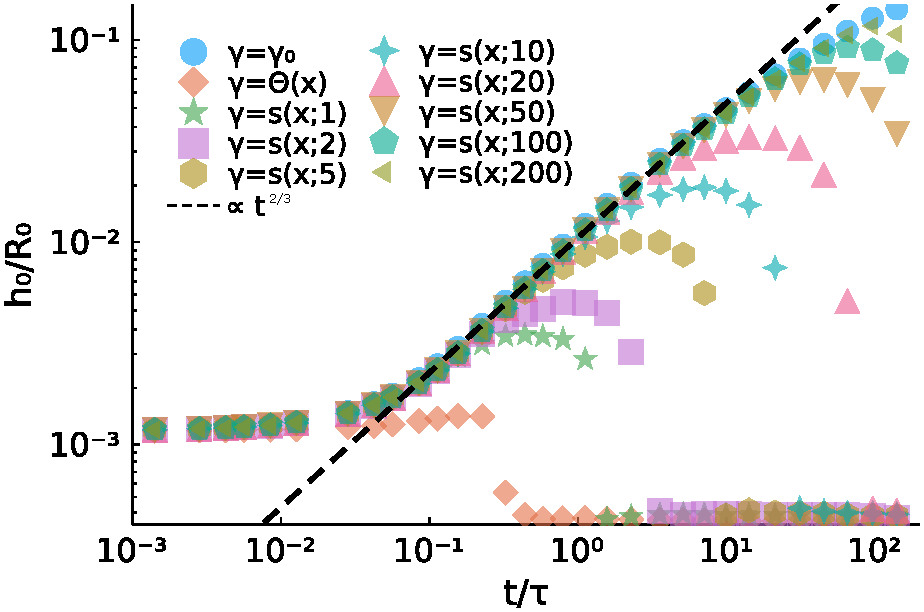
\includegraphics[width=0.48\textwidth]{Figures/bridge_evo_all_2.pdf}
    \caption{Time evolution of the liquid bridge $h_0(t)$ normalized with $R_0$. 
    Different symbols mark different surface tension gradients.
    The black dashed line displays $f(x) = \beta t^{2/3}$, with $\beta \approx 0.01$.}
    \label{fig:bridge_growth}
\end{figure}
First, let us introduce the parameters of our numerical experiments and the relevant length and time scales.
All experiments start with the same initial condition, two barely overlapping circular segments (equivalent to spherical caps in three dimensions) as illustrated in Fig.~\ref{fig:schematics}.
The grid size is $L=1024\Delta x$ with periodic boundary conditions except for $\partial_x\gamma(0) = \partial_x\gamma(L) = 0$.
Both droplets have a base radius $R_0 = 171\Delta x$, a maximum thickness $h_d = 30.15$ and form a contact angle $\theta = \pi/9$ with the substrate.
The initial bridge height is measured to be $h_0(0) \approx 0.2$.
The relaxation time $\tau = 1$ which in turn defines the viscosity to be $\mu = 1/6$. 
We use a slip boundary condition, see Eq.~(\ref{eq:fric_alpha}), with $\delta \approx h_0/2$.
The surface tension $\gamma_0 = 10^{-5}$, while $\Delta\gamma = 2\cdot 10^{-6}$.
In the disjoining pressure, Eq.~(\ref{eq:disjoin}) we set $h_{\ast} = 0.09$ and $(n,m) = (9,3)$.
% All quantities are given in $l.b.u$ so-called lattice Boltzmann units.

The length scale to nondimensionalize our results is the radius of the initial droplet $R_0$~\cite{PhysRevLett.111.144502, PhysRevLett.95.164503}.
Using this length scale a characteristic time scale is set by the inertio-capillary time 
\begin{equation}\label{eq:inertio-cap-time}
    \tau_{\text{ic.}} = \sqrt{\frac{\rho R_0^3}{\gamma}}.
\end{equation}
Inserting numbers yields a timescale $\tau_{\text{ic.}} \approx 7\cdot 10^5 \Delta t$ for $\gamma=\gamma_0$. 

\subsection{Bridge growth}\label{subsec:growth}
The liquid bridge between two similar drops on a solid substrate with contact angle $\theta < \pi/2$ is expected to grow according to Eq.~(\ref{eq:coal_powerlaw}). 
This powerlaw, $\alpha = 2/3$, holds true in our simulations where $\Pi(h) \neq 0$ shown by blue circles in Fig.~\ref{fig:bridge_growth}.
Only for late stages of the coalescence where $h_0 \sim h_d$ we observe a deviation from the black dashed line 
\begin{equation}\label{eq:fit_powerlaw}
    f(t) = \beta t^{2/3},
\end{equation}
with $\beta = 0.01$.
The powerlaw is however fairly dependent on the slippage $\delta$, because fluid needs to flow into the neck region.
For a $\delta \ll h_d$ this flow is suppressed, and therefore $\alpha < 2/3$.
 
Changing the $\gamma(x)$ changes the bridge growth quite severely.
Using Eq.~(\ref{eq:gamma_step}) instead of Eq.~(\ref{eq:gamma_const}) is shown by orange diamonds in Fig.~\ref{fig:bridge_growth}.
Clearly, the bridge does not grow, and the droplets do not coalesce.
This is in agreement with previous studies~\cite{karpitschka2014sharp, doi:10.1021/la500459v, PhysRevLett.109.066103, doi:10.1021/la800630w}. 
Including $\Pi(h) \neq 0$ the bridge even decreases, leaving only a thin precursor layer between the droplets.
Instead of a steady motion of the twin droplet state, we observe that the droplet on the lower surface tension side, therefore $\gamma_0 - \Delta\gamma$ moves away from the step. 
Resulting in a new equilibrium shape where $\partial_x\gamma = 0$.
This is expected because $\partial_x\gamma\neq 0$ induces a force which results in a flow, see Eq.~(\ref{eq:thin_with_marangoni}).

Smoothing out the surface tension gradient using Eq.~(\ref{eq:gamma_tanh}) is shown by the remaining symbols in Fig~\ref{fig:bridge_growth}.
Instead of an immediate separation of the droplets and independent of the smoothing width (different colors and symbols), the bridge starts to grow initially.
More surprisingly, the data is in agreement with the powerlaw $\propto t^{2/3}$ of Eq.~(\ref{eq:coal_powerlaw}).
The reason behind this flow is surface tension difference, the droplet on the higher surface tension side is sucking out fluid from the lower surface tension one.

\subsection{Asymmetry}\label{subsec:skewness}
\begin{figure}
    \centering
    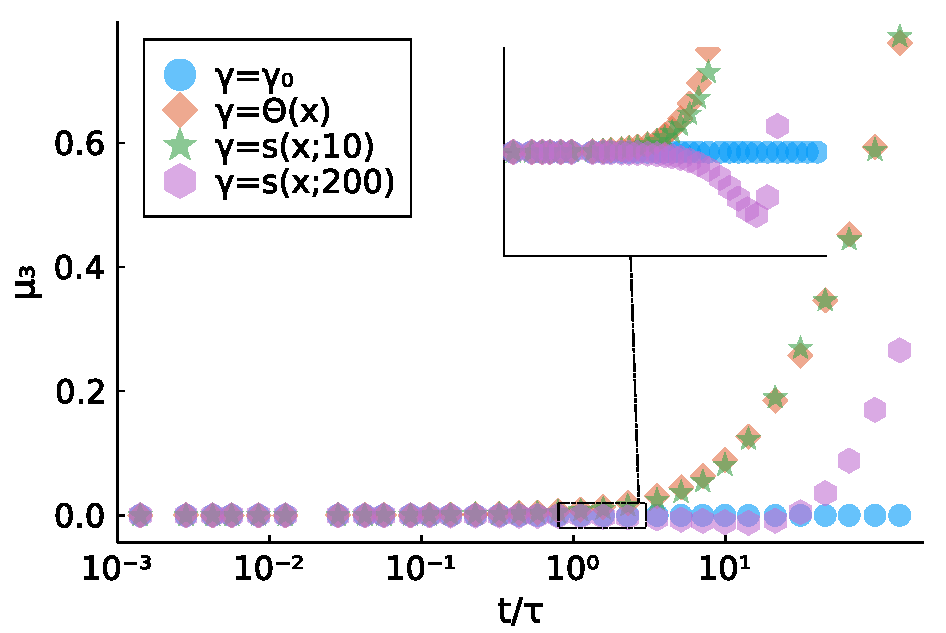
\includegraphics[width=0.48\textwidth]{Figures/skew_evo.pdf}
    \caption{Skewenss $\mu_3$ displayed during the time evolution for various surface tension gradients.}
    \label{fig:skewness}
\end{figure}

... see Fig.~\ref{fig:skewness}

\section{Summary and Conclusions}\label{sec:sum_conclu}
We have performed numerical simulations of coalescing droplets on a rigid substrate based on the thin film equation.
For droplets at small scales ($R \approx 1\mu m$) we assume that the disjoining pressure can not be neglected and therefore include it. 
The droplets are subject to a surface tension gradient that which is decoupled from the liquid.


\begin{acknowledgements}

\end{acknowledgements}
% \subsection{Comments Tilman}

% \begin{itemize}
%     \item \cite{doi:10.1021/la500459v} states that $\Pi(h)$ is neglectable. Maybe do simulations with and without disjoining pressure, that should be a matter of just commenting that part out. If you are lucky it runs stable without major issues and you can show that in your regime there indeed is a difference taking disjoining pressure into account, however big it turns out to be. 
    
%     \textcolor{pyblue}{Stefan}: It will not work.
%     There is an interface and ``dry'' spots, dry spots can only be done with disjoining pressure.
%     I tested this some time ago for some other reason.
    
%     My idea is to work out the modified equation with the inclusion of the disjoining pressure.
%     But feel free to work on it if you find it interesting.
    
%     Theory $>$ Simulation/Experiments!
    
%     \item Again \cite{doi:10.1021/la500459v}. In their experiment the surface tension gradient is induced by different liquids. In Figure 2 3b) you see the droplets in the non-coalesence case move thus the surface tension profile moves to. That may be worth to take into account.
    
%     \textcolor{pyblue}{Stefan}: Yeah I know.
%     The PRL~\cite{PhysRevLett.109.066103} kind of explains why, see Eqs.~(1,2,3).
% \end{itemize}

%\input{|python your_script.py}

%\appendix
%\section{}\label{app:one}

\bibliography{Ref}

\end{document}